\chapter{2Dcoupling\_algae: Algae 2D Coupling}
%

% - Purpose & Problem description:
%     These first two parts give reader short details about the test case,
%     the physical phenomena involved and specify how the numerical solution will be validated

\section{Purpose}

The purpose of this example is to show that for a test with algae, the algae dislodgement can be defined as a function of bed wave orbital velocity taken from a coupled TOMAWAC run.

\section{Description}

This test case is based on the TOMAWAC test case \textbf{3D coupling}, which is turn based on the SISYPHE test case \textbf{Littoral}.  Details of the flows and waves can be found in the documentation for these test cases.

\begin{figure}[h]%
	\begin{center}
		%
		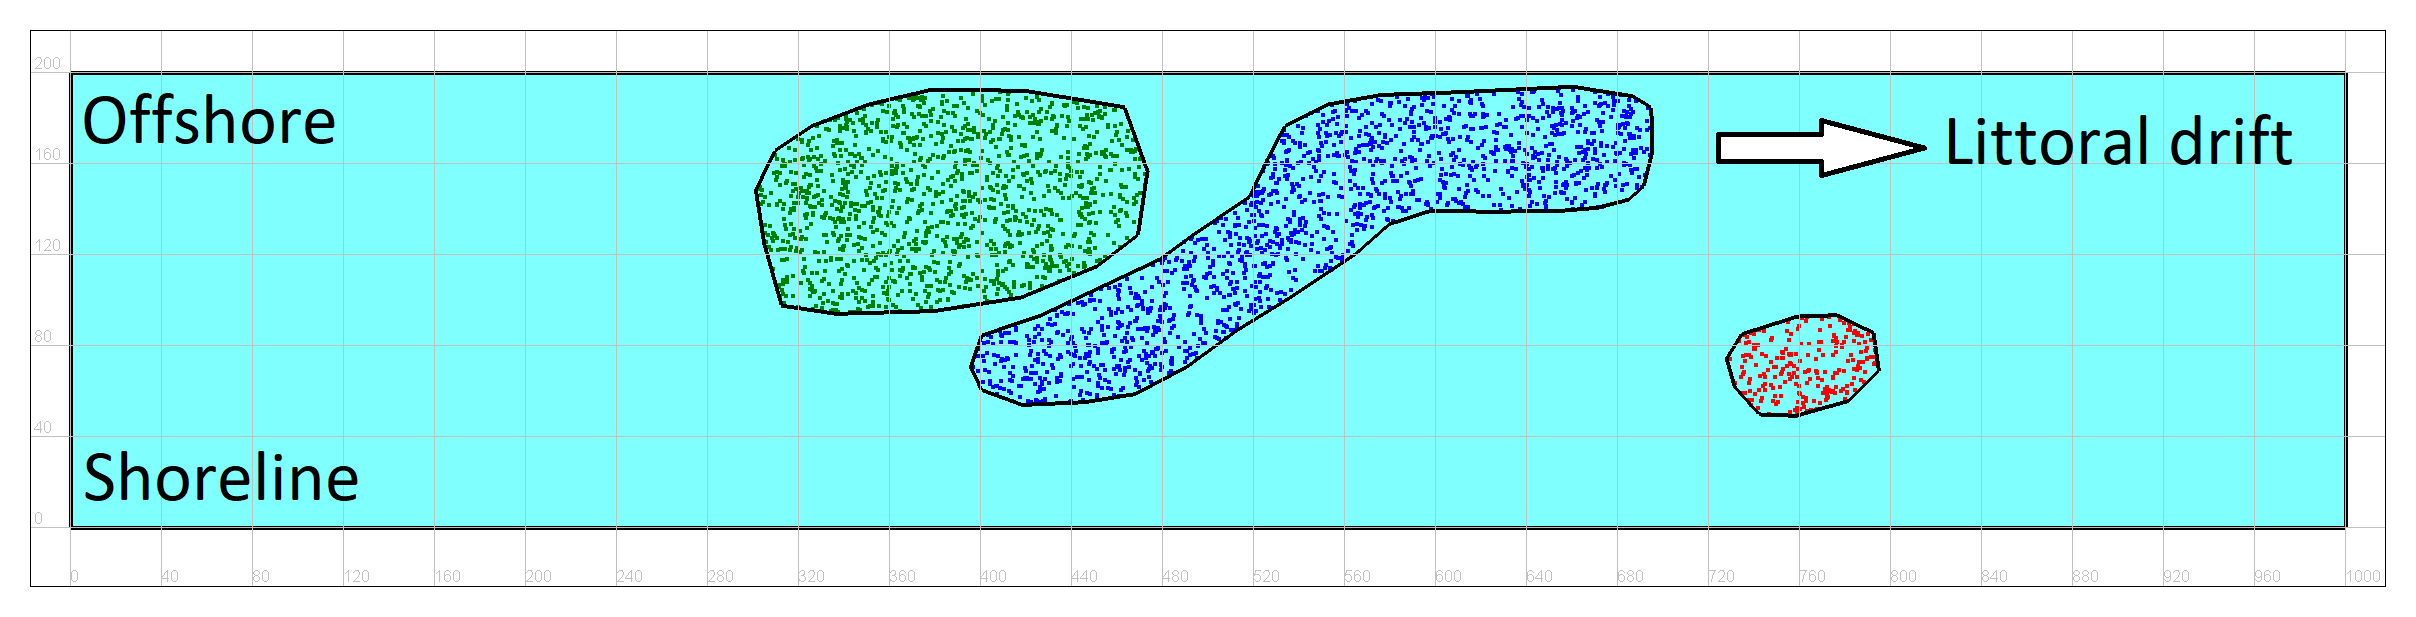
\includegraphics[width=0.75\textwidth]{./Figures/2Dcouple_initial_02}
		%
	\end{center}
	\caption{Initial algae distribution}
	\label{fig:exp2d_init}
\end{figure}

The initial algae distribution is defined using a polygon file, containing three polygons, which is specified using the keyword \texttt{DROGUES INITIAL POSITIONING DATA FILE}.   The polygon file must be in the BlueKenue i2s format.  The central polygon defines algae with class 1.  The left polygon defines algae with class 2.  The right polygon defines algae with class 3.

\smallskip
For this test case, the keyword \texttt{ALGAE RELEASE TYPE} equals 2 for all 3 classes.  This means an algae particle does not start to move until the wave orbital velocity at the bed exceeds a threshold value.  This option only works if the TELEMAC-2D run is coupled with TOMAWAC and if TOMAWAC supplies the wave orbital velocity to the TELEMAC-2D run.

\smallskip
The threshold value of the wave orbital velocity varies with time, according to the equation:
\begin{equation}
OV_0 = OV_1 + (OV_2 - OV_1) exp(-A . T_{eff})
\end{equation}

$OV_{1}$, $OV_{2}$ and $ A $ are specified in the steering file with the following keywords:

\begin{enumerate}
	\item[\nonumber] $OV_{1}$ = \textit{WAVE ORBITAL VELOCITY THRESHOLD FOR ALGAE 1}
	\item[\nonumber] $OV_{2}$ = \textit{WAVE ORBITAL VELOCITY THRESHOLD FOR ALGAE 2}
	\item[\nonumber] $A$ = \textit{RATE OF DEGRADATION FOR ALGAE}
\end{enumerate}
$T_{eff}$ is an “effective time” relating to the cumulative wave forcing that has been experienced by each algae particle, defined by: $T_{eff} = \sum { OV . dt}$ .  This means that $T_{eff}$ is the numerical integral of wave orbital velocity over time.

\smallskip
For this test, $OV_1 = 0.5 m/s$ for class 1, $0.7 m/s$ for class 2 and $0.4 m/s$ for class 3.
$A = 0.005$ for class 1 and class 2 and $0.01$ for class 3.

%
% - Results:
%     We comment in this part the numerical results against the reference ones,
%     giving understanding keys and making assumptions when necessary.
%
%
\section{Results}

\emph{Because of the turbulent particle movements the result on the reader's machine may be slightly different to the results below, but it should be similar.}

\smallskip
Figure~\ref{fig:res2d_3s} to Figure~\ref{fig:res2d_9s} show the algae distribution after 3 seconds, 6 seconds and 9 seconds.  

\smallskip
After 3 seconds, some of the central class 1 particles have been dislodged and have moved to the right.  This is because $OV_1$ is lower for the class 1 particles (blue)  than the class 2 particles (green), which have not yet been dislodged.  The class 3 particles (red) have not yet been dislodged because they are in a region of lower bed wave orbital velocity.

\smallskip
After 6 seconds, some of the class 2 particles have been dislodged.  This is because the critical bed wave orbital velocity has become lower, according to the equation given above.  In reality, the critical value would not change so quickly.  This test case can to the critical value changing quickly in order to illustrate the principle.

\smallskip
After 9 seconds, the particles have move further to the right and a wider band of particles have been dislodged.  The class 3 particles have been dislodged and have moved to the left slightly.

\begin{figure}[h]%
	\begin{center}
		%
		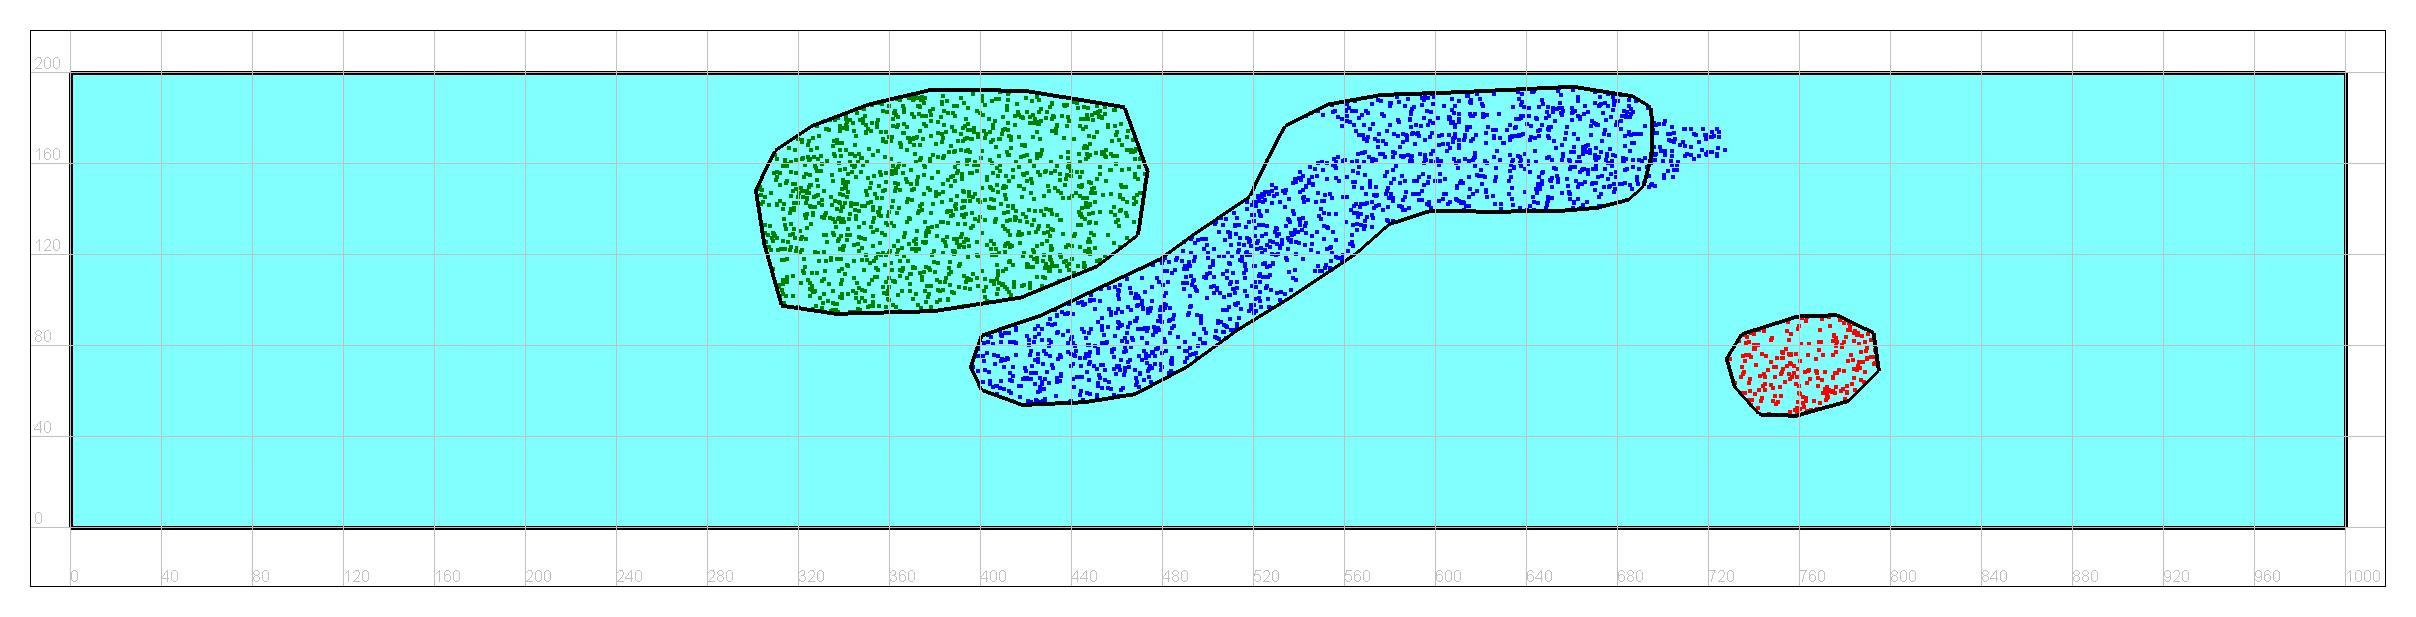
\includegraphics[width=0.75\textwidth]{./Figures/algae2dcouplingRes3s}
		%
	\end{center}
	\caption{Algae distribution after 3 seconds}
	\label{fig:res2d_3s}
\end{figure}

\begin{figure}[h]%
	\begin{center}
		%
		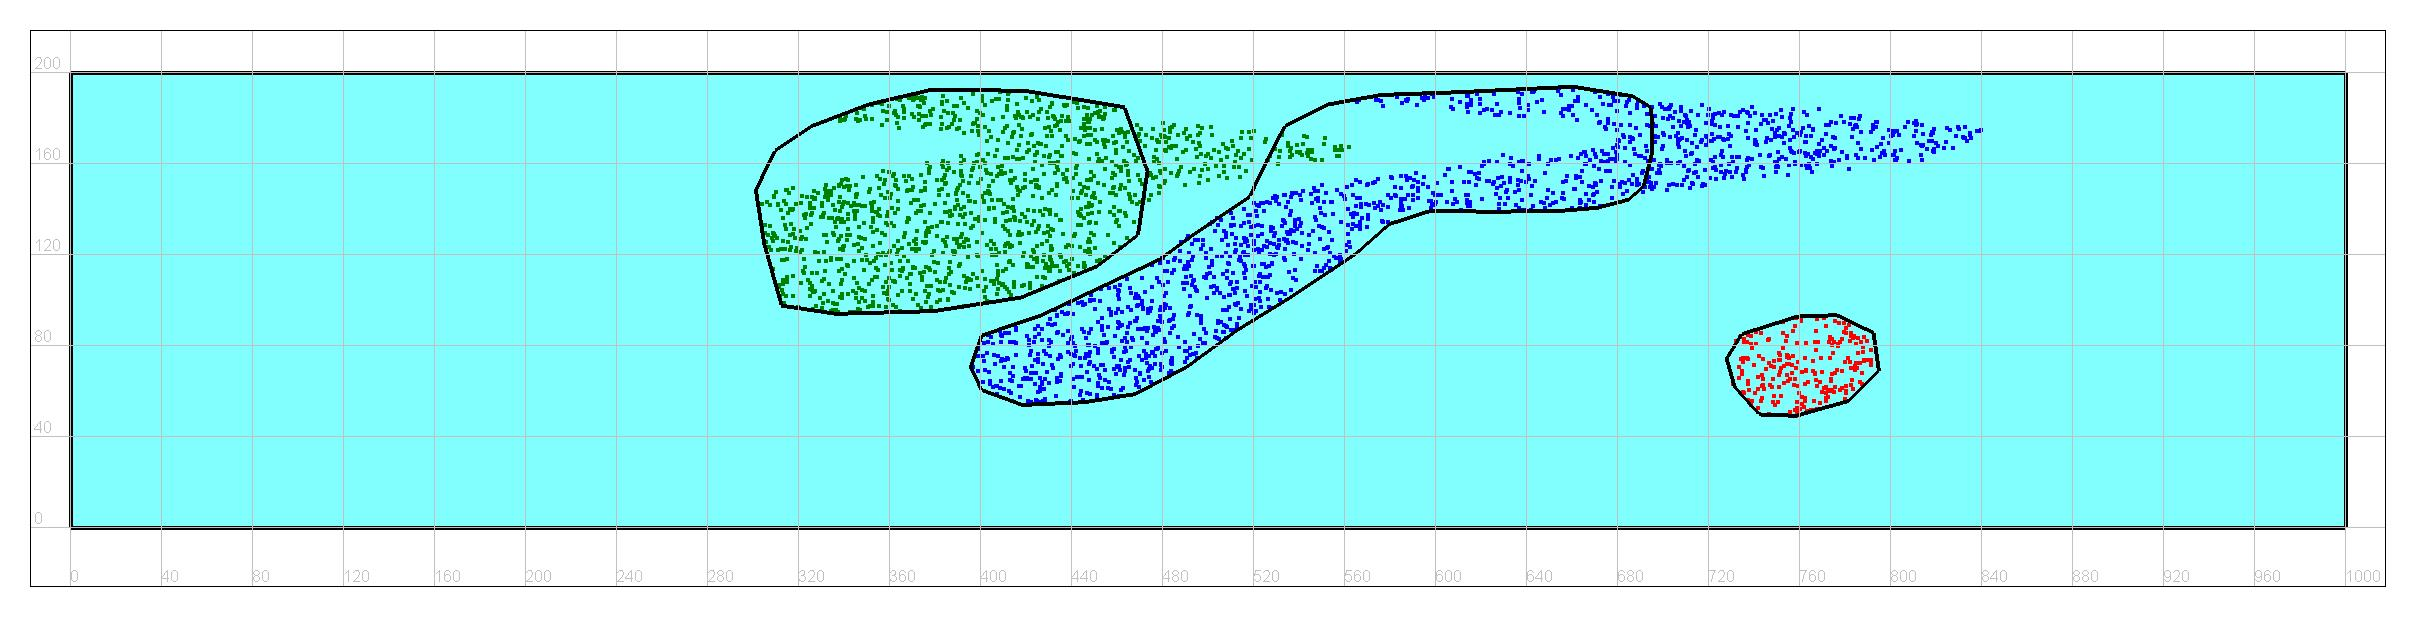
\includegraphics[width=0.75\textwidth]{./Figures/algae2dcouplingRes6s}
		%
	\end{center}
	\caption{Algae distribution after 6 seconds}
	\label{fig:res2d_6s}
\end{figure}

\begin{figure}[h]%
	\begin{center}
		%
		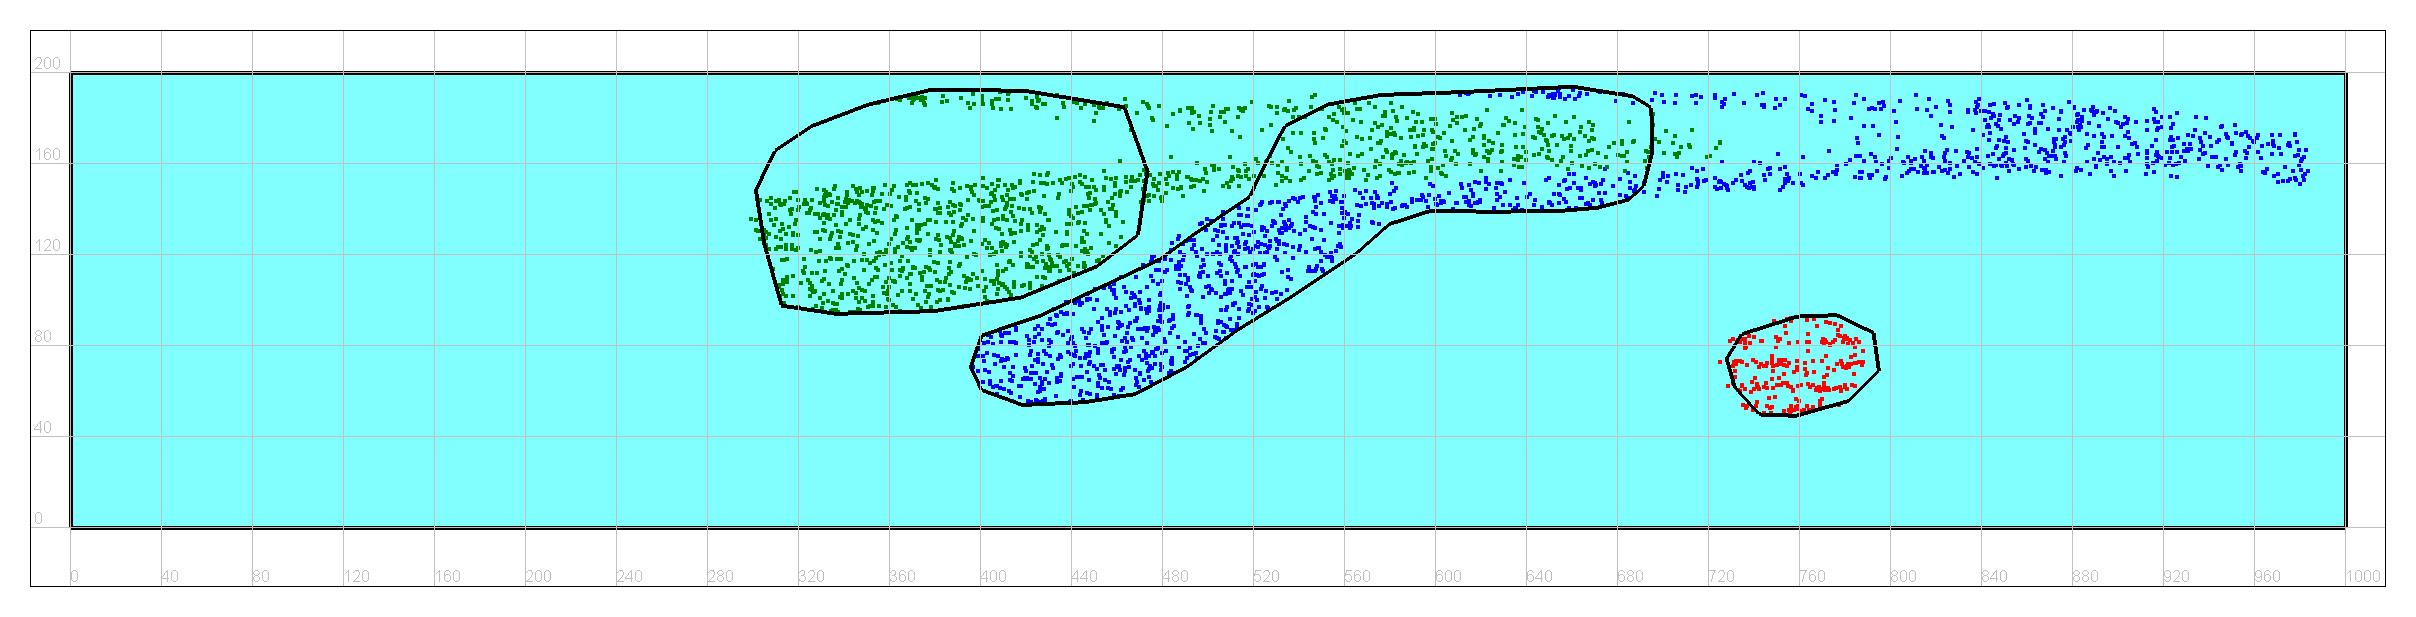
\includegraphics[width=0.75\textwidth]{./Figures/algae2dcouplingRes9s}
		%
	\end{center}
	\caption{Algae distribution after 9 seconds}
	\label{fig:res2d_9s}
\end{figure}

The standard test case outputs the algae information as a Tecplot file.  In this case the algae information is written to a file defined by the keyword \texttt{ASCII DROGUES FILE}.  The default value of the \texttt{DROGUES FILE FORMAT} is TECPLOT.  In order to output to a PCL file, give the output file name using the keyword \texttt{BINARY DROGUES FILE} and give the \texttt{DROGUES FILE FORMAT} as BKBINPCL.  PCL files can be displayed using BlueKenue.

\smallskip
This example outputs a text file called \verb!polygon_particles.txt!.  Output is written to the file every 10 seconds.  The output relates to the three polygons that define the three initial regions of particles, as described above.  
For each time, the output file contains the time, and the number of initial particles that remain in each polygon and un-mobilised.  Running of the test case should result in a text file identical to the \verb!polygon_particles.txt! file.

\smallskip
For this test case example the random distribution of initial particles is fixed through lines 39 to 47 of the \verb!condin_drogues.f! routine.  These lines ensure that the particles are initially located in the same place whenever the test case is run but should be commented out when running the code more generally.  

